\begin{figure}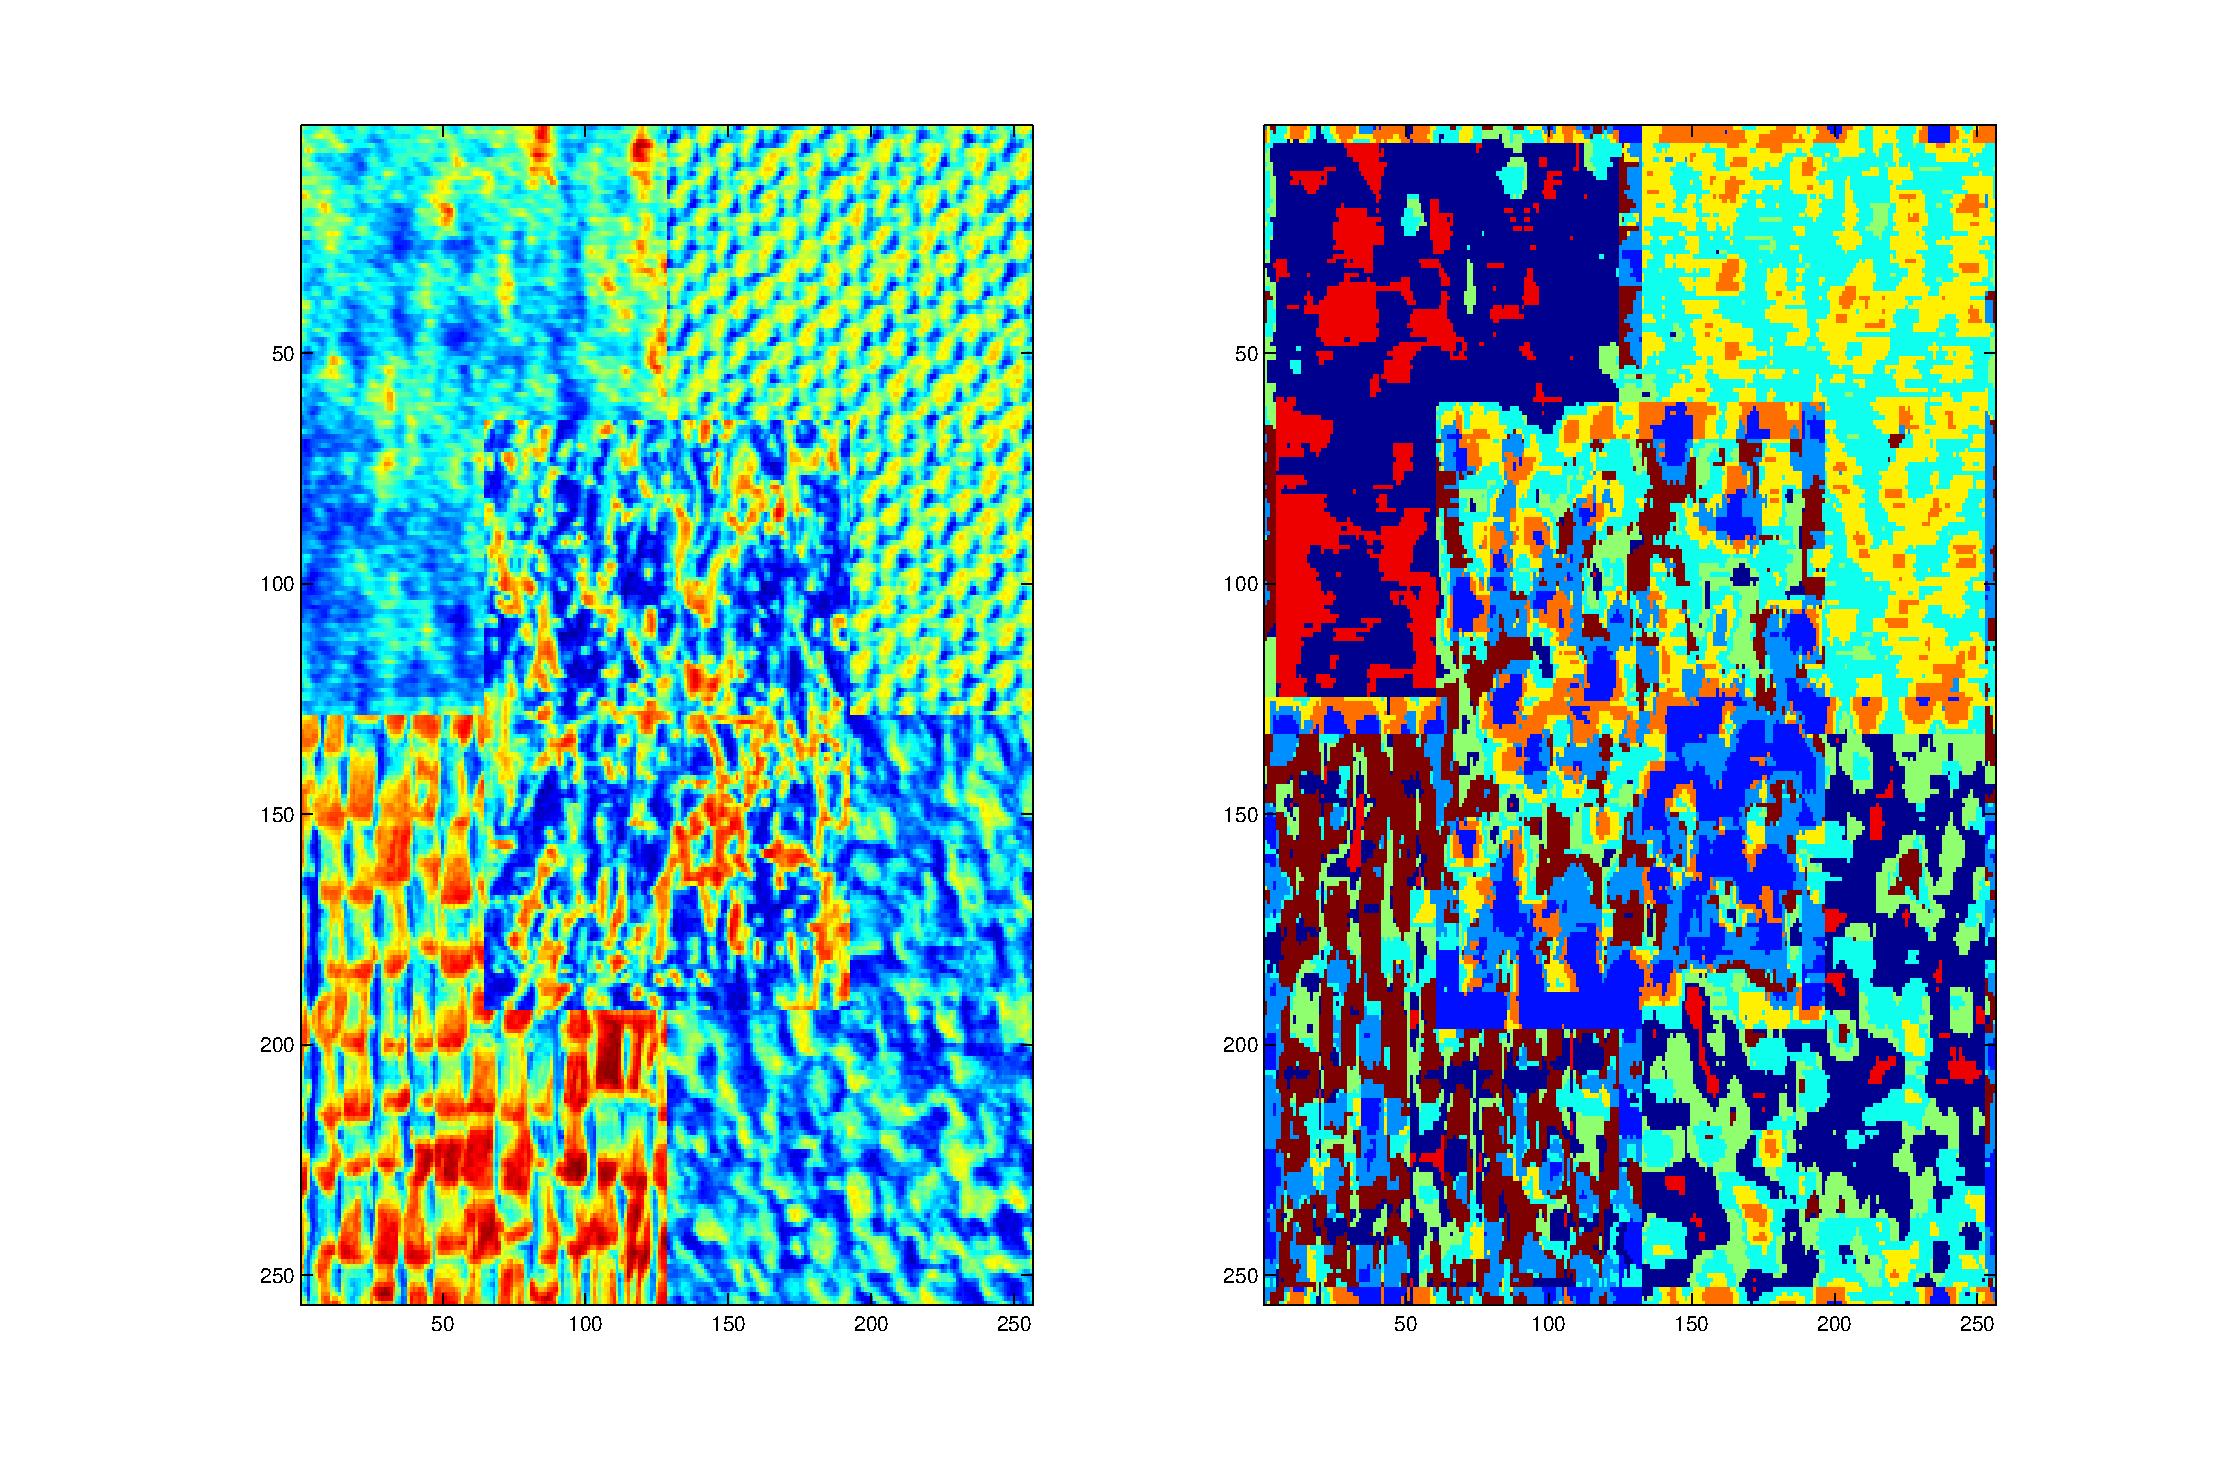
\includegraphics[width=\textwidth]{images/image-class}\label{fig:image-class}\caption{Results of Applying MICD Classifier to \textbf{multf8}}\end{figure}Firstly, the boundaries in the original texture image are well reflected in the classified region. 
Secondly, the cloth (top-left, dark blue) is quite often classified as stone (red). This is because the two classes are overlapped in the feature space. Cotton (top-right) is largely misclassified as pig-skin, cork and paper. Similarly, the classifiers for cork, raffia and grass do a poor job in terms of having a high misclassification rate. This is consistent with the confusion matrix in the Section 2.2.
Lastly, comparing cimage with original texture image multim, we find that there are some similarities between the two graphs. For example, the red part in the top left of cimage has similar shape of the corresponding dark region in the multim. Similarly, the good classification of raffia shows some pattern of vertical lines, which is also similar to the corresponding part of the multim. Therefore, the conclusion is that the classification indicates patterns of the original graph. This is intuitive since the classification is done to each block of the original graph. If the original graph has some pattern, that is, adjacent blocks are more or less similar, then it is very likely for them to be classified to the same class and show pattern in the classified graph.